\documentclass[english,11pt,twoside,a4paper]{article}
\usepackage[left=2cm,top=1cm,right=2cm,nohead,nofoot]{geometry}
\usepackage[utf8]{inputenc}
\usepackage{hyperref}
\usepackage{amssymb}
\usepackage{graphicx}
\begin{document}
\author{
  Niemistö, Jesse
  \and
  Muona, Leo
  \and
  Hilden, Matias
}
\title{Conceptual Design}

\maketitle

\section{Project idea}

Our aim in this project is to make a turret, which aims moving targets with laser pointer, and makes appropriate noises. This means that the turret will have following parts:

\begin{itemize}
  \item Raspberry Pi, the main controller. It holds the main software under Linux OS.
  \item Two DC motors (\url{http://www.kouluelektroniikka.fi/cgi-bin/shop.cg?action=prodshow\&usr=3qienj42dm87vuhhkuuv9nst84\&prodid=5561\%20545}), one for horizontal tracking and one for vertical tracking.
  \item Motor control circuit (L293D), which is able to control both motors.
  \item Camera (Raspberry Pi NoIR ccd camera module 5MPx), which is used for tracking movements.
  \item Circuit board, which is used for connections.
  \item Speaker (\url{http://www.partco.biz/verkkokauppa/product\_info.php?cath=17\_1440\_1916\&products\_id=1086})
  \item Audio amplifier, which is used with the speaker to produce audio output.
\end{itemize}

Our initial design consists of a static base, which has a horizontally rotating platform on top of it. This platform is rotated via one DC motor. On the platform we plan to mount the second DC motor, which has a laser pointer's base attached to it. This base is rotated vertically. Both DC motors are controlled by the Raspberry Pi via motor control circuit L293D.

We plan the software to have the following functionalities:

\begin{itemize}
  \item Movement detection via the camera.
  \item Greeting a person that is causing the movement with a common greeting.
  \item Aiming the laser pointer at the person that was detected.
  \item When movement has stopped, asking the person if he/she is still there.
  \item Playing extra sounds to make the turret more fun.
\end{itemize}

Inspiration for the project is from the game Portal by Valve Corporation. The game has white cute military turrets that try to kill the game's protagonist.

\begin{figure}
  \begin{center}
    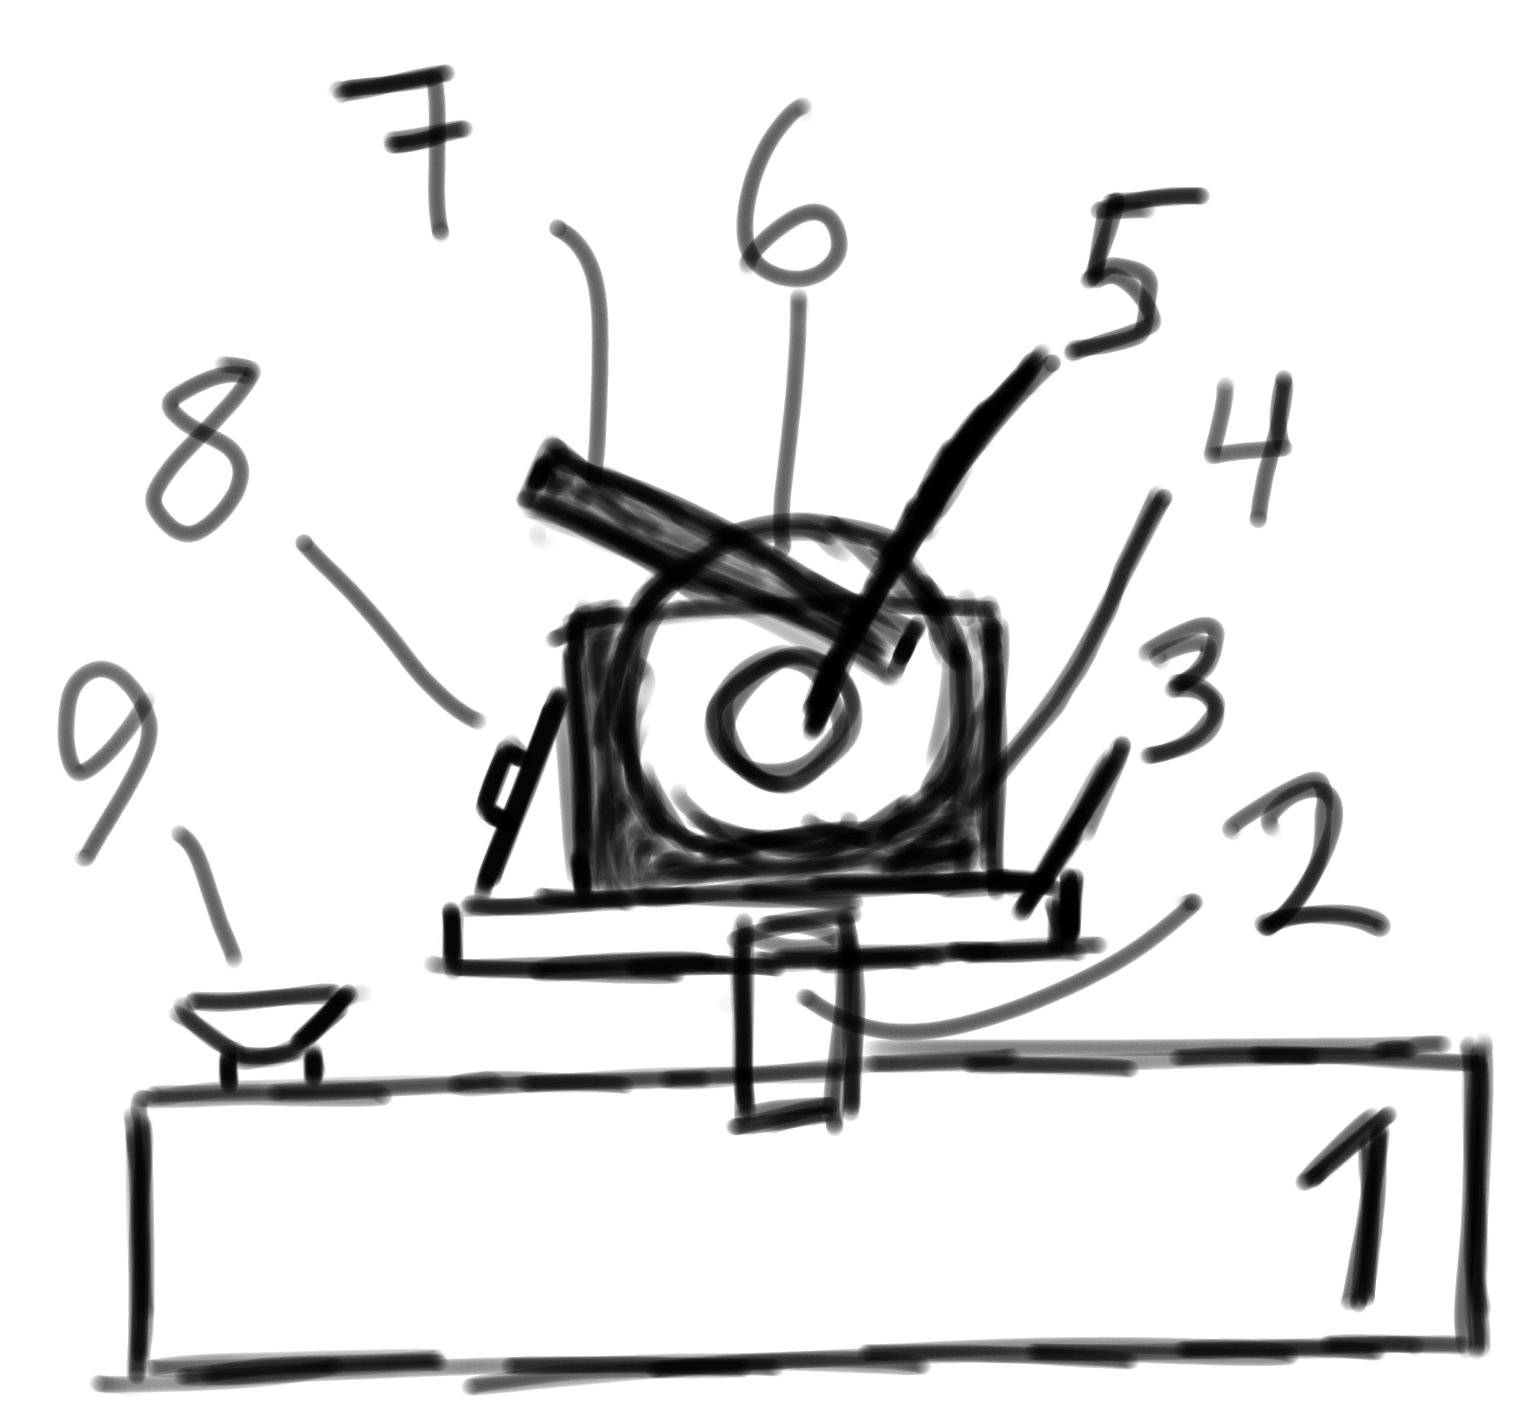
\includegraphics[scale=0.15]{design_sketch.png}
    \caption{Rough sketch of the design.}
  \end{center}
  \label{sketch}
\end{figure}

Figure~\ref{sketch} shows the rough design of the turret. The numbered parts are following.

\begin{enumerate}
  \item Raspberry pi, works also as the base for the turret.
  \item DC Motor.
  \item Platform that is rotated vertically by the DC motor of item 2.
  \item Random block of unknown material that is used as a base for item 5. Is attached to item 3.
  \item DC Motor, attached to block in item 4.
  \item Platform that is rotated horizontally by the DC motor of item 5.
  \item Pointing device (A Laser-like LED light), attached to platform of item 6.
  \item Camera unit, stands on top of platform of item 3.
  \item Speaker, on top of Raspberry pi.
\end{enumerate}

\section{Project timetable}

We plan to complete the project according to the following timetable.

\begin{itemize}
  \item Requirements and design: TODO
  \item Implementation: TODO
  \item Evaluation: TODO
  \item Demonstration: TODO
  \item Final report: TODO
\end{itemize}

\end{document}
